% !TEX program = xelatex
% Preview scope: Abstract, Introduction, System Model, Problem Formulation.
% Remaining section and subsection headings are deliberately empty.
\renewcommand{\rmdefault}{ptm}
\RequirePackage[T1]{fontenc}
\documentclass[conference]{IEEEtran}
\IEEEoverridecommandlockouts
\usepackage{mathptmx}
\usepackage{amsmath,amssymb,bm}
\usepackage{graphicx}
\usepackage{xcolor}
\usepackage[hidelinks]{hyperref}
\usepackage[capitalize,nameinlink,noabbrev]{cleveref}
\usepackage{microtype}
\newcommand{\UE}{\mathrm{UE}}
\newcommand{\BS}{\mathrm{BS}}
\newcommand{\EH}{\mathrm{EH}}
\newcommand{\DL}{\mathrm{DL}}
\newcommand{\RF}{\mathrm{RF}}
\newcommand{\fly}{\mathrm{fly}}
\newcommand{\hov}{\mathrm{hov}}
\newcommand{\tot}{\mathrm{tot}}
\newcommand{\setT}{\mathcal{T}_{\mathrm{s}}}
\newcommand{\setN}{\mathcal{N}}
\newcommand{\setM}{\mathcal{M}}
\newcommand{\norm}[1]{\left\lVert #1\right\rVert}
\interdisplaylinepenalty=2500
\pagestyle{plain}
\raggedbottom
\begin{document}
\title{Joint UAV Trajectory, NOMA Power Allocation and BS Deployment for Energy-Efficient SWIPT-Enabled Communications}
\author{Hoang Cao Minh, Ninh Thi Thanh Tam, Nguyen Minh Quan, and Trinh Van Chien
\thanks{Ninh Thi Thanh Tam is with the Faculty of Information and Communication Technology, National Academy of Education Management, Vietnam, and the School of Information and Communications Technology, Hanoi University of Science and Technology, Hanoi 100000, Vietnam (email: tam.ntt250098D@sis.hust.edu.vn).}
\thanks{Hoang Cao Minh, Nguyen Minh Quan, and Trinh Van Chien are with the School of Information and Communications Technology, Hanoi University of Science and Technology, Hanoi 100000, Vietnam (email: minh.hc2416559@sis.hust.edu.vn; quannm@soict.hust.edu.vn; chientv@soict.hust.edu.vn).}}
\maketitle
\thispagestyle{plain}

\begin{abstract}
Energy-efficient operation of a wireless communication UAV requires joint consideration of data delivery and the energy spent on flight, hovering, and radio transmission. This paper considers a SWIPT-enabled UAV-assisted downlink NOMA network in which multiple base stations supply radio-frequency energy to a rotary-wing UAV serving ground users. The UAV follows a horizontal trajectory at a fixed altitude and alternates between hovering for energy harvesting and data transmission, and cruising between consecutive service locations. We formulate a joint design of the UAV's horizontal waypoints, the NOMA power allocation coefficients, and the horizontal base-station deployment. The objective is to maximize the total delivered downlink bits per joule of UAV energy use, subject to user-specific mission data requirements, per-service-slot quality of service, deployment regions, directed trajectory progress, and an energy budget. The energy accounting explicitly includes propulsion during both cruise and hover, while harvested energy supplies the downlink RF load under an ideal conversion-and-use assumption. A particle-swarm-based framework, including an improved variant with adaptive mutation, is considered for the resulting nonconvex problem. The formulation exposes how communication gains from favorable channel geometry must be balanced against the propulsion cost of trajectory detours, and supports comparisons between fixed-infrastructure and joint-deployment designs.
\end{abstract}
\begin{IEEEkeywords}
UAV communications, energy efficiency, SWIPT, NOMA, trajectory optimization, base-station deployment, particle swarm optimization.
\end{IEEEkeywords}

\section{Introduction}
\label{sec:introduction}
An unmanned aerial vehicle (UAV) can provide a communication platform whose location changes with the spatial distribution of ground users. This mobility is useful when terrestrial coverage is incomplete or temporary service is required. By approaching a favorable service location, the UAV can improve the channels to its users. Reaching that location, however, also consumes propulsion energy. Consequently, a communication design must account for the energy cost of mobility as well as the amount of information delivered. For a rotary-wing UAV that communicates while hovering, the service duration introduces an additional propulsion load even when the UAV is stationary.

Power-domain non-orthogonal multiple access (NOMA) allows several users to share a downlink resource through superposition coding and successive interference cancellation (SIC). Its power allocation must account for the users' channel conditions and the interference remaining at each decoding stage. Simultaneous wireless information and power transfer (SWIPT) provides another design mechanism: a UAV can harvest energy from the signals transmitted by ground base stations (BSs) and use that energy for downlink RF transmission. In such a network, the UAV position affects both the BS-to-UAV energy supply and the UAV-to-user transmission rates. The horizontal deployment of the BSs further shapes the available RF power over the mission.

The relationship between flight and communication energy has been studied explicitly in UAV communications. \href{https://arxiv.org/abs/1804.02238}{Zeng, Xu, and Zhang (2018)} develop a rotary-wing propulsion model and optimize a UAV's trajectory and communication schedule under individual data requirements.\footnote{Y. Zeng, J. Xu, and R. Zhang, \emph{Energy Minimization for Wireless Communication with Rotary-Wing UAV}, arXiv:1804.02238, 2018. \url{https://arxiv.org/abs/1804.02238}.} Their fly-hover-communicate design makes the service-location and travel-energy trade-off explicit. In a related SWIPT-enabled NOMA setting, \href{https://doi.org/10.1109/VTC2024-Fall63153.2024.10758018}{Baduge, Perera, and Jayakody (2024)} use particle swarm optimization (PSO) to design UAV positions for a minimum-rate objective.\footnote{D. P. P. R. Baduge, T. D. P. Perera, and D. N. K. Jayakody, \emph{Flight to Efficiency: Trajectory Optimization in SWIPT-Enabled UAV-Assisted NOMA for Future Wireless Networks}, IEEE VTC2024-Fall, 2024, doi: 10.1109/VTC2024-Fall63153.2024.10758018.} These studies motivate a design that places downlink data delivery and UAV energy use within a common mission-level objective.

Trajectory and power control also arise in NOMA-assisted backscatter networks. \href{https://doi.org/10.3390/drones10040238}{Zhang et al. (2026)} jointly address UAV data-collection locations, trajectory, power allocation, and reflection coefficients under an energy budget.\footnote{T. Zhang, M. Gu, D. Mishra, J. Yuan, and A. Seneviratne, \emph{Trajectory and Power Control for Sustainable UAV-Assisted NOMA-Enabled Backscattering IoT}, Drones, vol. 10, no. 4, article 238, 2026, doi: 10.3390/drones10040238.} Their setting involves backscatter data collection; the present work considers active UAV-to-user downlink transmission powered by harvested RF energy. We use its multirotor propulsion model and include hovering energy during service.

The design considered here is driven by two coupled requirements. First, a trajectory detour can improve the energy-harvesting link, the downlink channels, or both, but increases the distance flown. Second, maximizing aggregate data delivery alone can leave individual users underserved. A mission-level data requirement protects each user's total payload, while a per-user requirement in every service slot prevents temporary service starvation. BS positions are selected once for the mission and affect all service locations; they therefore couple the trajectory and power allocation decisions across the complete route.

We address these requirements through a joint trajectory, NOMA allocation, and BS deployment formulation. The UAV altitude, cruising speed, hovering duration, power-splitting ratio, and harvesting efficiency are prescribed. Both horizontal UAV coordinates are optimized, subject to fixed endpoints and minimum directed progress along the mission axis. BS heights remain fixed, whereas their horizontal coordinates may vary within admissible deployment regions. The resulting design is evaluated by the ratio of total downlink payload to the combined cruise, hover, and RF energy used by the UAV.

The main contributions of this work are as follows:
\begin{itemize}
\item We formulate a mission-level bits-per-joule objective that combines a harvest-then-transmit service protocol with explicit cruise and hover propulsion costs. This accounting distinguishes total UAV energy use from ideal battery expenditure.
\item We jointly design horizontal UAV waypoints, ordered NOMA power shares, and static BS deployment under individual mission payload requirements, slot-level service thresholds, geometric restrictions, and an overall energy budget.
\item We establish a PSO-based search framework and an improved variant with stagnation-dependent mutation for this coupled design. Fixed-BS and joint-deployment configurations provide a basis for examining the roles of trajectory freedom, infrastructure placement, and the search procedure.
\end{itemize}

\section{System Model}
\label{sec:system_model}
\subsection{Network Geometry and Mission Structure}
Consider one rotary-wing UAV, $M$ ground BSs indexed by $\setM=\{1,\ldots,M\}$, and $N$ ground users indexed by $\setN=\{1,\ldots,N\}$. User $n$ has a fixed position $\bm u_n=[x_n^{\UE},y_n^{\UE},0]^T$. BS $m$ is located at $\bm b_m=[x_m^{\BS},y_m^{\BS},z_m^{\BS}]^T$, where $z_m^{\BS}$ is fixed and $\bm s_m=[x_m^{\BS},y_m^{\BS}]^T$ is selected within a prescribed rectangle $\mathcal B_m$. Deployment is an offline planning decision: a BS remains at the selected location during the UAV mission.

\begin{figure*}[t]
\centering
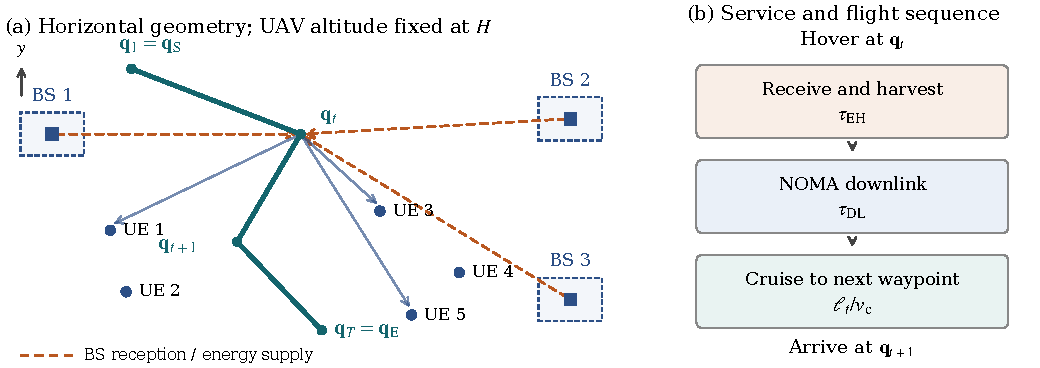
\includegraphics[width=\textwidth]{Images/system_model.pdf}
\caption{Illustrative network geometry and mission protocol. BS horizontal positions are selected within deployment regions (dashed rectangles). The UAV serves users while hovering, with reception/harvesting followed by NOMA downlink transmission, and then cruises to the next waypoint. The geometry is schematic, not an optimized simulation outcome.}
\label{fig:1SystemModel}
\end{figure*}
The network and its service protocol are illustrated in \cref{fig:1SystemModel}.

The UAV route comprises $T$ ordered waypoints,
\begin{equation}
\bm q_t=[x_t,y_t,H]^T,\qquad t=1,\ldots,T,
\label{eq:waypoints}
\end{equation}
at a constant altitude $H>0$. The first and last positions are fixed at $\bm q_{\mathrm S}$ and $\bm q_{\mathrm E}$, respectively. The service-slot set is
\begin{equation}
\setT=\{1,\ldots,T-1\}.
\label{eq:internal_steps}
\end{equation}
At each $t\in\setT$, the UAV hovers at $\bm q_t$, completes its communication service, and then flies to $\bm q_{t+1}$. Thus the initial waypoint is a service location, while the final waypoint is an arrival point with no additional service interval. Every flight segment, including the one entering the final waypoint, contributes to the energy and duration of the mission.

Each hover interval lasts $\tau_{\hov}>0$ and is divided into a BS reception/energy-harvesting phase and a downlink transmission phase:
\begin{equation}
\tau_{\EH}=\lambda\tau_{\hov},\qquad
\tau_{\DL}=(1-\lambda)\tau_{\hov},\quad 0<\lambda<1.
\label{eq:phase_times}
\end{equation}
These durations are fixed and common to all service slots. Communications occur at the hovering locations; no payload is credited during flight. With prescribed horizontal cruise speed $v_{\mathrm c}>0$, the segment distance, flight time, and mission duration are
\begin{align}
\ell_t&=\norm{\bm q_{t+1}-\bm q_t},\quad
\tau_t^{\fly}=\ell_t/v_{\mathrm c},\label{eq:flight_time}\\
T_{\mathrm{mission}}&=\sum_{t\in\setT}\tau_t^{\fly}
+(T-1)\tau_{\hov}.\label{eq:mission_time}
\end{align}
The service-slot index therefore does not denote a fixed-duration flight slot. A longer segment increases the actual mission duration through \cref{eq:flight_time}.

\subsection{Air-to-Ground Channel Model}
\label{subsec:channel_assumptions}
For either a BS or a user at $\bm a_i=[a_{i,x},a_{i,y},a_{i,z}]^T$, define the horizontal separation, link distance, and elevation magnitude as
\begin{align}
d_{t,i}&=\sqrt{(x_t-a_{i,x})^2+(y_t-a_{i,y})^2},\nonumber\\
r_{t,i}&=\sqrt{d_{t,i}^2+(H-a_{i,z})^2},\nonumber\\
\theta_{t,i}&=\operatorname{atan2}(|H-a_{i,z}|,d_{t,i}).
\label{eq:distances}
\end{align}
All modeled links have $r_{t,i}>0$, and $\theta_{t,i}\in[0,\pi/2]$. The use of a vertical-separation magnitude also covers a BS whose height equals or exceeds the UAV altitude. The large-scale power gain is
\begin{equation}
\beta_{t,i}=\beta_0\left(\frac{r_{t,i}}{r_0}\right)^{-\nu},
\qquad r_0=1\ \mathrm m,
\label{eq:path_loss}
\end{equation}
where $\beta_0$ is the reference gain and $\nu$ is the path loss exponent.

The small-scale coefficient follows an elevation-dependent Rician construction:
\begin{align}
K_{t,i}&=A_1\exp(A_2\theta_{t,i}),\label{eq:rician_k}\\
g_{t,i}&=\sqrt{\frac{K_{t,i}}{K_{t,i}+1}}\,\bar g
+\sqrt{\frac{1}{K_{t,i}+1}}\,\widetilde g_i,
\label{eq:rician_fading}
\end{align}
where $\bar g=1$, $\widetilde g_i\sim\mathcal{CN}(0,1)$, $A_1=K_{\min}$, and $A_2=(2/\pi)\ln(K_{\max}/K_{\min})$. The $K$-factor endpoints are expressed in linear scale. Separate scattering samples are drawn for the physical BS and user links. Within one scenario, each $\widetilde g_i$ is held fixed across waypoints and candidate designs; the geometry-dependent path loss and Rician mixture still change with the UAV and BS positions. This defines a deterministic, realization-conditioned mission design rather than an optimization of ergodic rates.

Combining the propagation components gives the UAV-to-user and BS-to-UAV coefficients
\begin{equation}
h_{t,n}=\sqrt{\beta_{t,n}^{\UE}}\,g_{t,n}^{\UE},\qquad
k_{t,m}=\sqrt{\beta_{t,m}^{\BS}}\,g_{t,m}^{\BS}.
\label{eq:channels}
\end{equation}
User positions, BS heights, and the channel realization are assumed available for offline design. No independent shadowing process or inter-cell downlink interference is included.

\subsection{SWIPT Reception and Harvested-Energy Use}
Every BS transmits with prescribed power $P^{\BS}$ during the reception phase. Independent BS signals give the aggregate received RF power
\begin{equation}
P_{t}^{\mathrm{rec}}=P^{\BS}\sum_{m\in\setM}|k_{t,m}|^2.
\label{eq:received_power}
\end{equation}
With fixed power-splitting fraction $\varphi\in[0,1]$ routed to the harvesting branch and linear conversion efficiency $\eta\in[0,1]$, the harvested energy is
\begin{equation}
E_t^{\EH}=\eta\varphi P_t^{\mathrm{rec}}\tau_{\EH}.
\label{eq:harvested_energy}
\end{equation}
All of this energy is used for downlink RF transmission in the same service slot, yielding
\begin{equation}
P_t=\frac{E_t^{\EH}}{\tau_{\DL}}
=\eta\varphi P^{\BS}\frac{\tau_{\EH}}{\tau_{\DL}}
\sum_{m\in\setM}|k_{t,m}|^2.
\label{eq:uav_power}
\end{equation}
Thus $P_t$ is determined by the geometry and harvesting parameters; it is not an independently optimized transmit-power variable. The phase-duration ratio in \cref{eq:uav_power} is required even though it equals one when the two phases have equal duration.

The information branch is assumed to provide sufficient data for the modeled downlink payload. The present model does not impose a BS-to-UAV decoding-rate constraint or a two-hop information-causality constraint. Accordingly, the payload metric quantifies downlink delivery under this data-availability assumption. The harvesting model includes neither saturation nor storage losses, and RF power-amplifier and circuit loads are omitted. Harvested energy supplies the RF load; propulsion is supplied by the onboard battery.

\subsection{Downlink NOMA and Delivered Payload}
At service slot $t$, let $\pi_t$ order the physical users from weakest to strongest channel:
\begin{equation}
|h_{t,\pi_t(1)}|^2\le\cdots\le|h_{t,\pi_t(N)}|^2.
\label{eq:sic_order}
\end{equation}
For brevity, $[u]=\pi_t(u)$ denotes a rank in this slot only. User $n$ receives power share $\alpha_{t,n}$, so its transmitted RF power is $P_t\alpha_{t,n}$. The normalized shares follow the weak-to-strong ordering
\begin{equation}
\sum_{n\in\setN}\alpha_{t,n}=1,\qquad
\alpha_{t,[1]}\ge\cdots\ge\alpha_{t,[N]}\ge0.
\label{eq:allocation}
\end{equation}
The UAV transmits a superposition of unit-power user symbols. Under ideal SIC, a user cancels the messages of weaker users and treats stronger-user messages as interference. Its SINR and achievable rate are
\begin{align}
\gamma_{t,[u]}&=
\frac{P_t\alpha_{t,[u]}|h_{t,[u]}|^2}
{\sigma^2+P_t|h_{t,[u]}|^2\sum_{j=u+1}^{N}\alpha_{t,[j]}},
\label{eq:sinr}\\
R_{t,n}&=B\log_2(1+\gamma_{t,n}),
\label{eq:rate}
\end{align}
where $B$ is the bandwidth and $\sigma^2=N_0B$ is the receiver noise power for noise spectral density $N_0$ in linear units. The interference sum is zero for $u=N$. Common receiver noise and the channel ordering allow a stronger user to decode a weaker user's message at the rate supported by that weaker user, under the ideal-SIC assumption.

The payload of physical user $n$ in slot $t$, its mission payload, and the aggregate mission payload are respectively
\begin{align}
D_{t,n}&=\tau_{\DL}R_{t,n},\label{eq:slot_bits}\\
D_n&=\sum_{t\in\setT}D_{t,n},\qquad
D_{\tot}=\sum_{n\in\setN}D_n.
\label{eq:total_bits}
\end{align}
These quantities are measured in bits. All mission data requirements are indexed by physical user identity, even if its channel rank changes along the route. No bits are counted at the final arrival waypoint.

\subsection{Propulsion and Mission Energy Accounting}
We use the steady horizontal multirotor power expression of Zhang et al. (2026), with thrust interpreted as the magnitude of the rotor force required to balance drag and weight. At horizontal speed $v$, let
\begin{equation}
F_{\mathrm d}(v)=\tfrac12\rho S_{\mathrm{FP}}v^2,\qquad
T_{\mathrm r}(v)=\frac{\sqrt{(mg)^2+F_{\mathrm d}(v)^2}}{n_{\mathrm r}},
\label{eq:thrust}
\end{equation}
where $m$ is UAV mass, $g$ is gravitational acceleration, $\rho$ is air density, $S_{\mathrm{FP}}$ is the equivalent fuselage flat-plate area, and $n_{\mathrm r}$ is the number of rotors. The total propulsion power is
\begin{equation}
P_{\mathrm{prop}}(v)=P_{\mathrm{pro}}(v)
+P_{\mathrm{ind}}(v)+P_{\mathrm{par}}(v),
\label{eq:propulsion}
\end{equation}
with blade-profile, induced, and parasite components
\begin{align}
P_{\mathrm{pro}}(v)&=\frac{n_{\mathrm r}\delta}{8}
\left(\frac{T_{\mathrm r}(v)}{c_T\rho A}+3v^2\right)
\sqrt{\frac{T_{\mathrm r}(v)\rho c_s^2 A}{c_T}},
\label{eq:profile}\\
P_{\mathrm{ind}}(v)&=n_{\mathrm r}(1+c_f)T_{\mathrm r}(v)
\left(\sqrt{\frac{T_{\mathrm r}(v)^2}{4\rho^2A^2}
+\frac{v^4}{4}}-\frac{v^2}{2}\right)^{1/2},
\label{eq:induced}\\
P_{\mathrm{par}}(v)&=\tfrac12n_{\mathrm r}d_0\rho c_sAv^3.
\label{eq:parasite}
\end{align}
Here $A$ is the disc area of one rotor; $c_s$, $\delta$, and $c_T$ denote rotor solidity, blade-section drag coefficient, and thrust coefficient; $c_f$ is the induced-power correction; and $d_0$ is the fuselage drag ratio. Hover power follows from the same model at zero speed, $P_{\hov}=P_{\mathrm{prop}}(0)$, while cruise power is $P_{\mathrm c}=P_{\mathrm{prop}}(v_{\mathrm c})$. Transient acceleration, braking, turning, and vertical-flight costs are outside the steady-flight approximation.

The three mission energy components are
\begin{align}
E_{\fly}&=P_{\mathrm c}\sum_{t\in\setT}\frac{\ell_t}{v_{\mathrm c}},\label{eq:flight_energy}\\
E_{\hov}&=P_{\hov}(T-1)\tau_{\hov},\label{eq:hover_energy}\\
E_{\RF}&=\sum_{t\in\setT}P_t\tau_{\DL}
=\sum_{t\in\setT}E_t^{\EH}.
\label{eq:rf_energy}
\end{align}
Hover propulsion is counted throughout both reception and transmission, since the UAV must remain airborne during each phase. The total energy-use metric is
\begin{equation}
E_{\tot}=E_{\fly}+E_{\hov}+E_{\RF}.
\label{eq:total_energy}
\end{equation}
The harvested energy is the source of $E_{\RF}$ and is not added again to \cref{eq:total_energy}. Under the ideal source assignment, the battery supplies $E_{\mathrm{bat}}=E_{\fly}+E_{\hov}$. We nevertheless include RF energy in $E_{\tot}$ to measure the complete modeled UAV load, irrespective of its energy source. Neither BS transmit energy nor BS circuit energy is included; the resulting efficiency is therefore a UAV-side energy-use metric.

\section{Problem Formulation}
\label{subsec:problem_formulation}
\subsection{Design Variables and Energy Efficiency}
The design variables are the internal horizontal UAV waypoints, the service-slot power allocation matrix, and the horizontal BS deployment:
\begin{equation}
\mathcal X=\{\bm Q,\bm A_{\alpha},\bm S\},
\label{eq:variable_set}
\end{equation}
where $\bm Q=\{(x_t,y_t)\}_{t=2}^{T-1}$, $\bm A_{\alpha}=[\alpha_{t,n}]_{t\in\setT,n\in\setN}$, and $\bm S=\{\bm s_m\}_{m\in\setM}$. Heights, phase durations, BS transmit powers, the power-splitting fraction, and cruise speed remain prescribed. For $E_{\tot}>0$, the objective is
\begin{equation}
\mathrm{EE}_{\mathrm{UAV}}(\mathcal X)
=\frac{D_{\tot}(\mathcal X)}{E_{\tot}(\mathcal X)}
\quad[\mathrm{bit/J}].
\label{eq:ee_objective}
\end{equation}
This is a ratio of mission totals, rather than an average of individual slot efficiencies. It also differs from either an RF-only or a battery-only efficiency.

\subsection{Joint Constrained Design}
Let $\mathcal R=[x_{\min},x_{\max}]\times[y_{\min},y_{\max}]$ be the horizontal flight region and set $s_y=\operatorname{sign}(y_{\mathrm E}-y_{\mathrm S})$, with $y_{\mathrm E}\ne y_{\mathrm S}$. Each segment must make at least $\Delta_y>0$ progress toward the endpoint along the mission axis. Denote by $L_n$ the minimum mission payload of user $n$, by $d_n^{\min}$ its minimum payload in each service slot, and by $d_{\Sigma}^{\min}$ an optional aggregate slot requirement. An overall UAV energy-use budget is denoted by $E_{\max}$. The joint problem is
\begin{subequations}
\label{eq:P1}
\begin{align}
(\mathrm{P1}):\quad
\max_{\mathcal X}\quad&\frac{D_{\tot}}{E_{\tot}}
\label{eq:P1_obj}\\
\mathrm{s.t.}\quad
&\bm q_1=\bm q_{\mathrm S},\quad\bm q_T=\bm q_{\mathrm E},
\label{eq:c_endpoints}\\
&(x_t,y_t)\in\mathcal R,\quad z_t=H,\label{eq:c_region}\\
&s_y(y_{t+1}-y_t)\ge\Delta_y,\label{eq:c_progress}\\
&\bm s_m\in\mathcal B_m,\label{eq:c_bs}\\
&\sum_{n\in\setN}\alpha_{t,n}=1,\label{eq:c_alpha}\\
&\alpha_{t,\pi_t(u)}\ge\alpha_{t,\pi_t(u+1)},\label{eq:c_noma}\\
&\alpha_{t,n}\ge0,\label{eq:c_alpha_positive}\\
&D_n\ge L_n,\label{eq:c_payload}\\
&D_{t,n}\ge d_n^{\min},\label{eq:c_user_slot}\\
&\sum_{n\in\setN}D_{t,n}\ge d_{\Sigma}^{\min},\label{eq:c_slot}\\
&E_{\tot}\le E_{\max}.
\label{eq:c_budget}
\end{align}
\end{subequations}
Waypoint constraints apply to $t=1,\ldots,T$, service and segment constraints to $t\in\setT$, BS constraints to $m\in\setM$, and user constraints to $n\in\setN$. In \cref{eq:c_noma}, $u=1,\ldots,N-1$.
The rates, available RF powers, distances, and energies in $(\mathrm{P1})$ are defined by \cref{eq:flight_time,eq:channels,eq:uav_power,eq:sinr,eq:rate,eq:slot_bits,eq:total_bits,eq:total_energy}; they are dependent quantities rather than additional free variables.

\Cref{eq:c_endpoints,eq:c_region} set the mission boundaries and constant flight altitude. \Cref{eq:c_progress} enforces directed progress in either mission direction; it does not require equally spaced waypoints. A necessary endpoint compatibility condition is $(T-1)\Delta_y\le|y_{\mathrm E}-y_{\mathrm S}|$. The BS rectangles in \cref{eq:c_bs} are fixed before optimization, and the selected BS positions are shared by all slots.

\Cref{eq:c_alpha,eq:c_noma,eq:c_alpha_positive} describe normalized, ordered NOMA allocation. In a numerical search, bounded positive auxiliary weights can be normalized and assigned in descending order to the ascending channel ranks. Bounds on these raw weights are numerical parameterization choices; they must not be interpreted directly as lower or upper bounds on the normalized power shares.

\Cref{eq:c_payload} protects the total data service of each physical user. \Cref{eq:c_user_slot} additionally protects service in every individual slot, which a mission-total requirement alone cannot ensure. \Cref{eq:c_slot} permits a separate aggregate slot threshold; setting a threshold to zero disables its corresponding nonnegative-payload restriction. \Cref{eq:c_budget} constrains the gross UAV energy-use metric in \cref{eq:total_energy}, including the RF load supplied by harvested energy. This budget and the objective use the same energy scope.

\subsection{Coupling and Solution Scope}
The problem couples communication and motion through the mission geometry. A waypoint change affects both sets of channels, the RF power supplied by \cref{eq:uav_power}, and the distances to neighboring waypoints. A BS relocation changes the harvested energy available at all service locations. The NOMA allocation determines the distribution of payload across users and must satisfy requirements at both mission and slot scales. For fixed geometry, $E_{\RF}$ is independent of the NOMA shares, whereas the achieved rates and individual data feasibility still depend on those shares.

Because the number and duration of hover intervals are prescribed, $E_{\hov}$ is constant across candidate designs within a configuration. Nevertheless, it remains in the bits-per-joule denominator and in the energy budget. Cruise energy changes with route length, while RF energy changes with the harvesting geometry. Consequently, maximizing harvested energy or sum rate alone does not in general maximize \cref{eq:ee_objective}.

The fractional objective, geometry-dependent propagation, NOMA interference, and channel-order-dependent allocation make $(\mathrm{P1})$ nonconvex in general. Changes in channel rank also change the assignment between ordered power shares and physical user identities. These features motivate a population-based search for feasible designs without asserting global optimality. Fixing $\bm S$ produces the fixed-BS joint trajectory/allocation case; optimizing all of $\mathcal X$ produces the full joint-deployment case. Both use the same payload definitions, energy accounting, and feasibility tests.

\section{Proposed Algorithms}
\label{sec:algorithms}
\subsection{Overview of the Proposed Joint Optimization Framework}
\label{subsec:algorithm_overview}
\subsection{Solution Representation}
\label{subsec:solution_representation}
\subsection{Fitness Function Design}
\label{subsec:fitness_function}
\subsection{Constraint Handling and Solution Repair}
\label{subsec:constraint_handling}
\subsection{Joint PSO-Based Optimization}
\label{subsec:joint_pso}
\subsection{Improved PSO Variant}
\label{subsec:improved_pso}

\section{Experimental Results}
\label{sec:results}

\section{Conclusion}
\label{sec:conclusion}

\section*{References}
\end{document}
